 \subsection{Database}
The figure \ref{fig:database} below shows how the database is structured. 

\clearpage
\begin{figure}[H]
	%\centering
	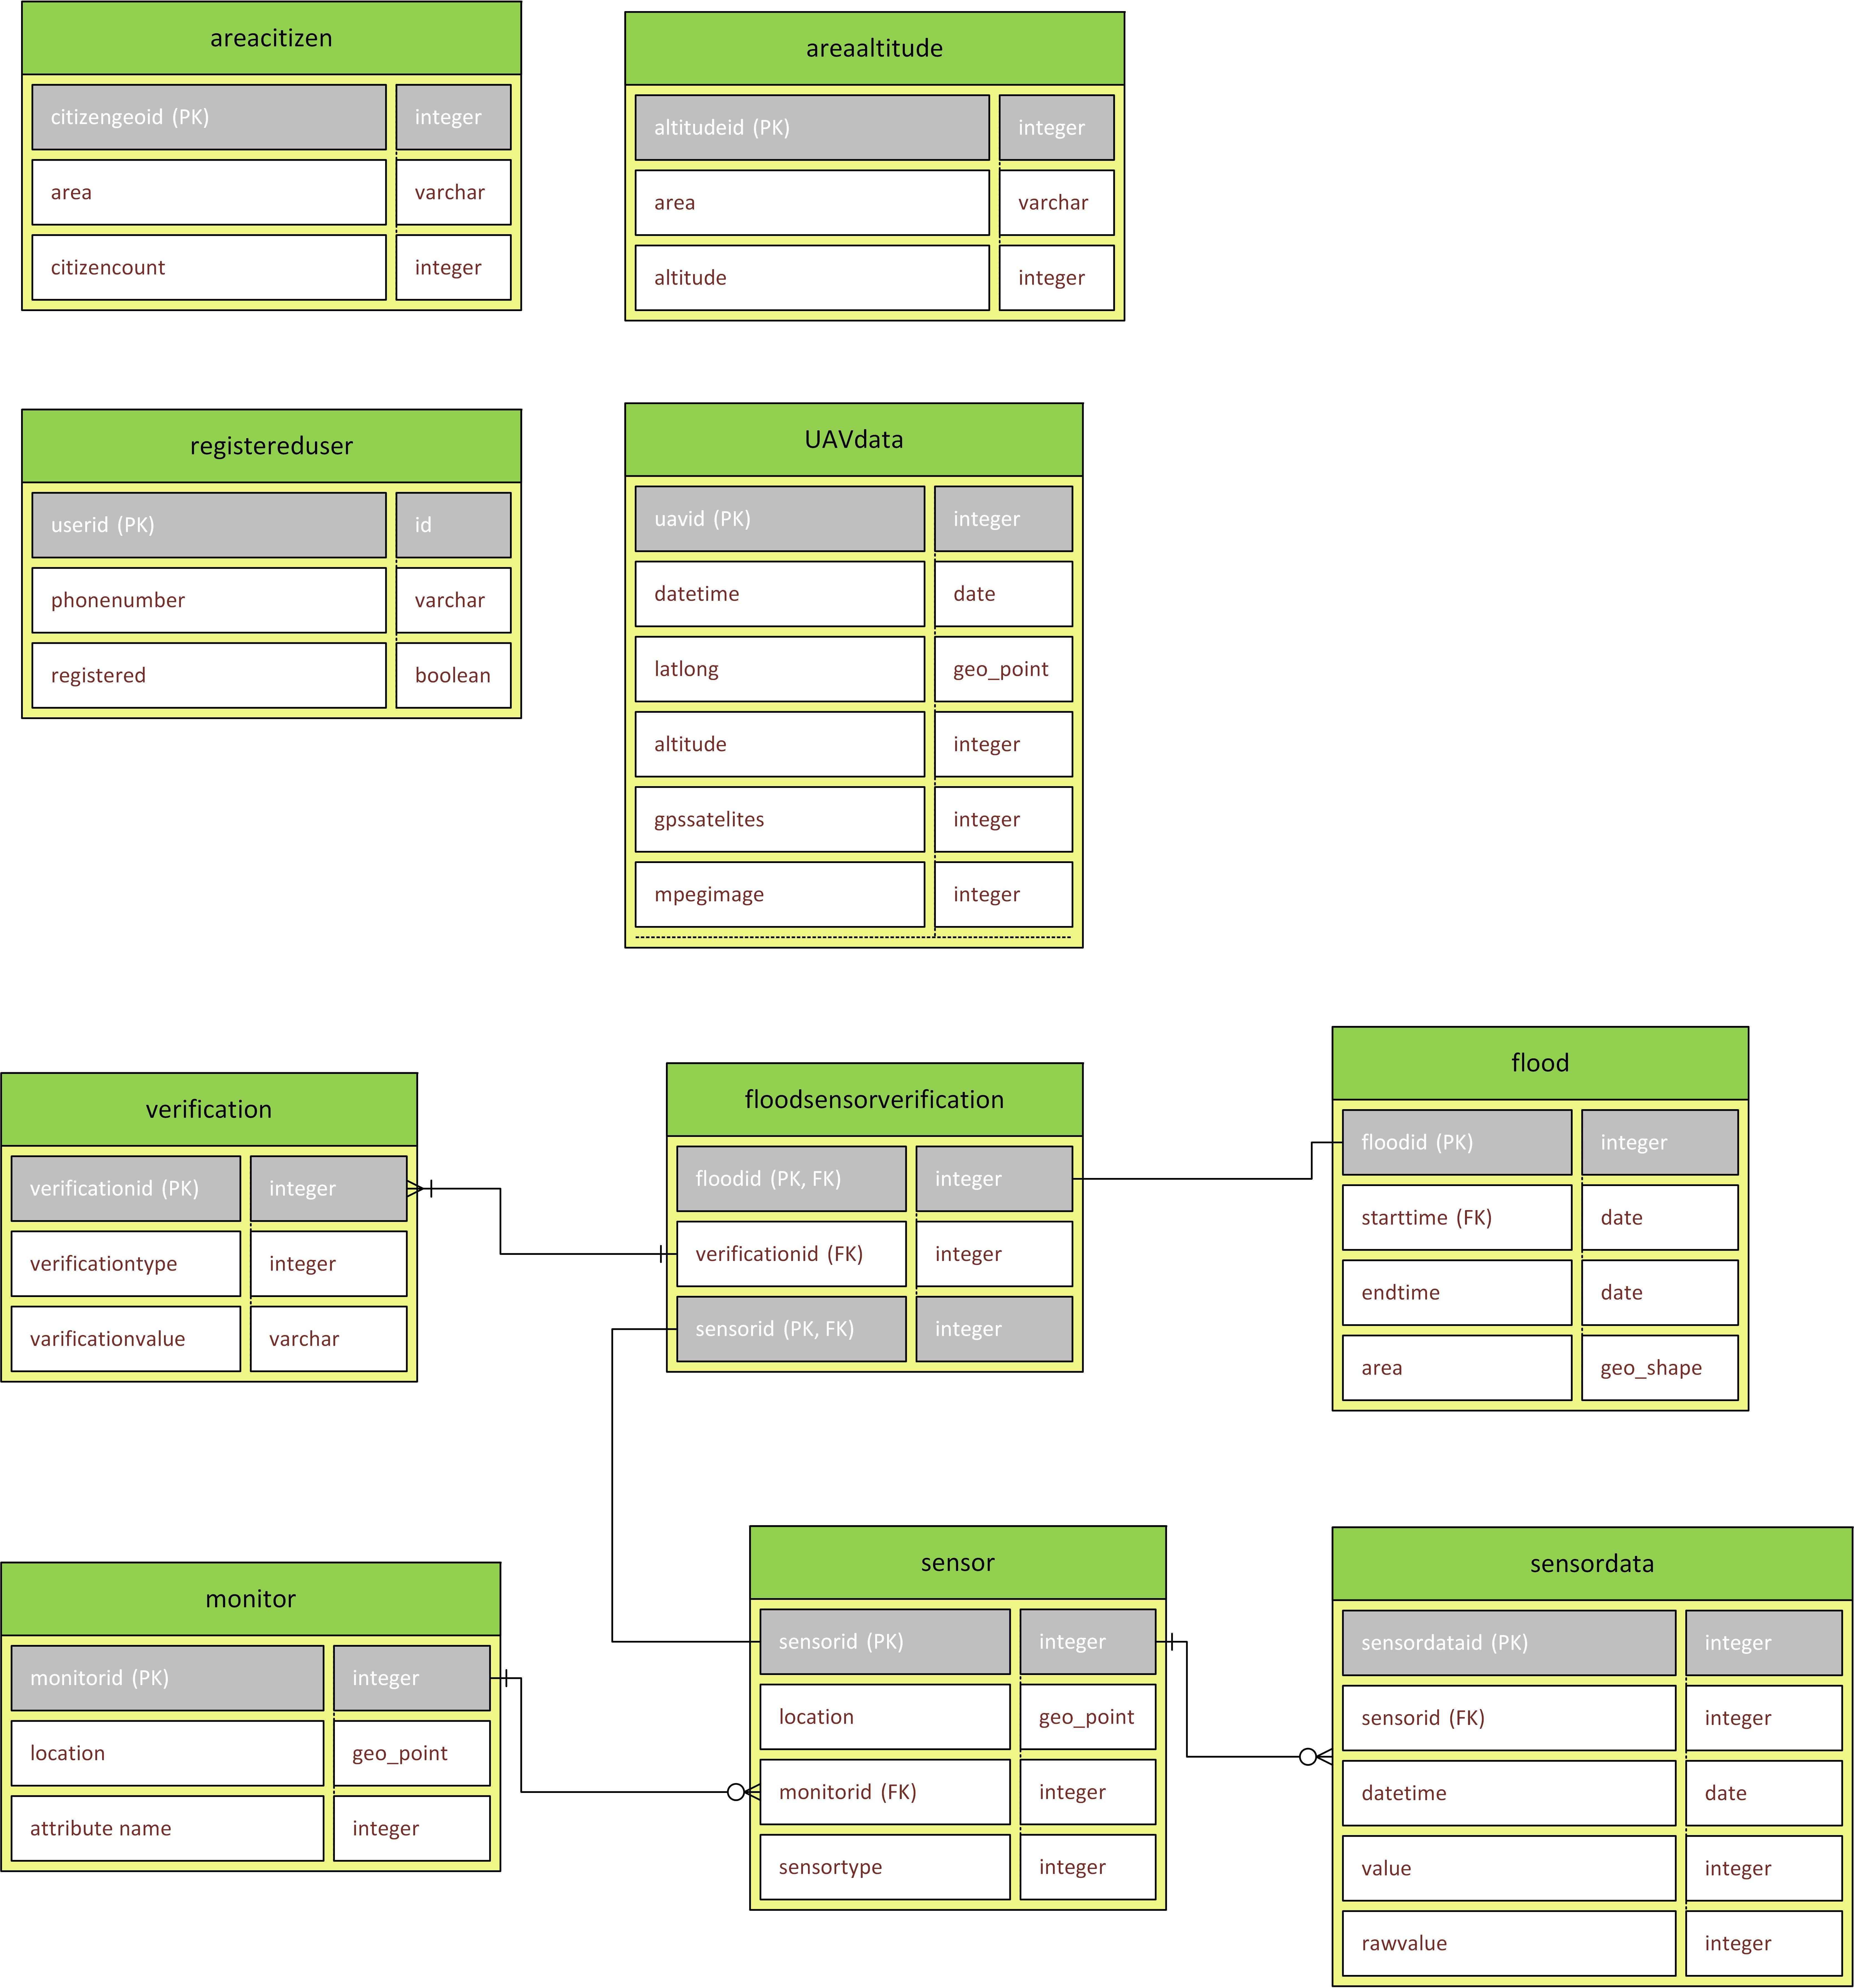
\includegraphics[height=14cm, width=0.9\textwidth]{{\viewimages/database}.jpg}
	\caption{Database diagram}
	\label{fig:database}
\end{figure}

The database diagram shows all the information the API can provide to the users. \\
The database is made of ten tables. \\

In green is the name of the table. \\
In grey the primarykey. \\
In the second column of each table are the types of the data. \\

The first table \textbf{aeracitizen} concerns the area where live the citizens : citizengeold (?) , area : the name of the area and citizencount gives the number of citizen in this area.\\
The table \textbf{aeraaltitude} gives information about the are such as its altitude.
The table \textbf{UAVdata} provides information sent by the UAVs which will give more information about the flood such as : uavid which identifies a specific uav, datetime, altitude , latlong ,gpssatelite,mpegimage, \\
The table \textbf{registereduser} concerns information to identify a specific user to provide him the warning, provide guidance and help the safety region : his id, phonenumer and if he is registered or not. \\

Six table are related and provide information about the sensors : \\
verification (?) \\
The table \textbf{Floodsensorverification} (?) \\
The table \textbf{flood}gives information about the flood : its id by floodid , starttime , endtimide , area. \\
The table \textbf{monitor} : monitorid , its location, attributename. \\
The table \textbf{sensor} : sensorid identifies each sensor, its location , which monitor it depends on,and its type \\
The table \textbf{sensordata} : sensordataid which identifies each data of the sensor, sensorid, datetime which gives the exact time of when the data has been sent ,value,  rawvalue(?). 

